\section{Применение метода сухого электронно-лучевого травления для формирования синусоидальных голографических решеток}

Проведенные эксперименты показали, что при экспонировании резиста в процессе СЭЛТР ``в кадр'' профиль получаемого рельефа имеет волнообразную форму.
Вследствие этого целесообразным является изучение возможности использования метода СЭЛТР для формирования синусоидальных голографических решеток, широко использующихся в оптике и получаемых в основном методом интерференционной литографии~\cite{Harrison2004_sin_gratings, Tishchenko2017_sin_gratings}.
Характерными параметрами таких решеток являются плотность штрихов порядка 1000 1/мм и глубина рельефа порядка 100 нм~\cite{Harvey2020_diffraction_gratings}.

Было проведено моделирование профиля рельефа, получаемого методом СЭЛТР при экспонировании ``в кадр'' c числом линий в кадре, равным 625, и отношением длины кадра к его ширине 1.3:1.
Расстояние между линиями варьировалось от 0.5 до 2 мкм, температура образца и ток экспонирования были приняты равными 150~$^\circ$C и 4.56 нА соответственно, начальная толщина слоя ПММА составляла 500 нм.
В свою очередь, диаметр пучка, время экспонирования и скорость охлаждения образца после экспонирования подбирались для получения профиля, максимально близкого к синусоидальному.
Результаты моделирования представлены на рисунках~\ref{fig:DEBER_holo_2um}, \ref{fig:DEBER_holo_1um} и \ref{fig:DEBER_holo_0p6um}.

На основании результатов моделирования можно заключить, что методом СЭЛТР могут быть получены синусоидальные голографические решетки с периодом до 0.5 мкм, что соответствует плотности штрихов 2000 1/мм.
Как показано на рисунке~\ref{fig:DEBER_holo_2um}, рельеф с синусоидальным профилем может быть получен как при полном или частичном наличии микрополостей в слое резиста (рисунки~\ref{fig:DEBER_holo_2um}a, ~\ref{fig:DEBER_holo_2um}б), так и при их отсутствии (рисунки~\ref{fig:DEBER_holo_2um}в, ~\ref{fig:DEBER_holo_2um}г).
При начальной толщине слоя ПММА, равной 500 нм, глубина рельефа может составлять от 0 до 200 нм в зависимости от концентрации микрополостей в слое ПММА.
При этом среднеквадратичное отклонение промоделированных профилей от графика функции синус составляет менее 5\% от глубины решетки.
Полученные в \linebreak ПММА синусоидальные решетки могут быть в дальнейшем покрыты металлом или перенесены в металл путем травления в реакторе индуктивно-связанной плазмы~\cite{Bruk_2016_mee}, что обеспечит формирование отражательной синусоидальной голографической решетки.

% 2 um
\begin{figure}[t!]
	\begin{minipage}{0.48\textwidth}
			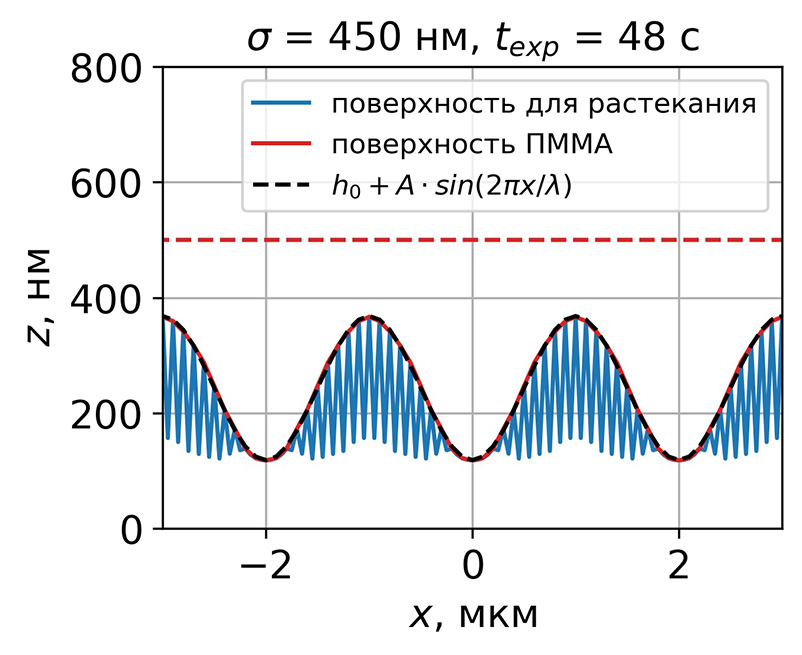
\includegraphics[width=\linewidth]{DEBER_holo/2_um/holo_1C_s450_48s_um_200} \\
			\vspace{-13em} \\ \text{\hspace{0em} a}) \\ \vspace{13em}
		\end{minipage}
	\begin{minipage}{0.48\textwidth}
			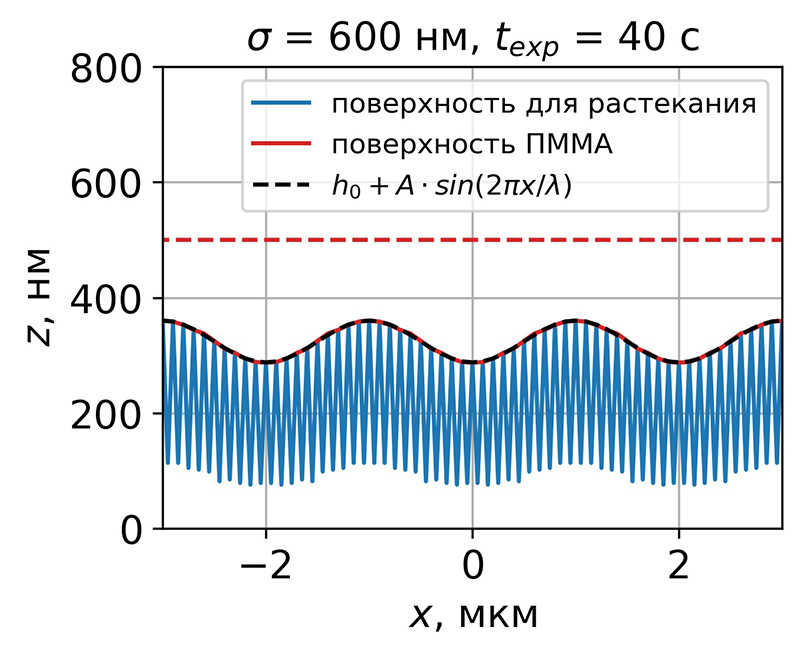
\includegraphics[width=\linewidth]{DEBER_holo/2_um/holo_1C_s600_40s_um_200} \\
			\vspace{-13em} \\ \text{\hspace{-0.1em} б}) \\ \vspace{13em}
		\end{minipage}
	
	\vspace{-3em}
	
	\begin{minipage}{0.48\textwidth}
			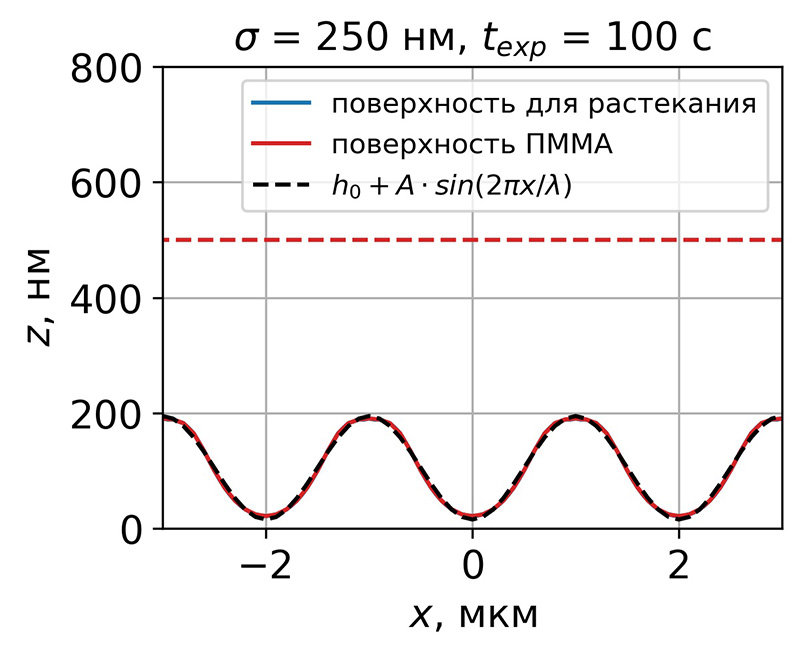
\includegraphics[width=\linewidth]{DEBER_holo/2_um//holo_10C_s250_100s_um_200} \\
			\vspace{-13em} \\ \text{\hspace{0em} в}) \\ \vspace{13em}
		\end{minipage}
	\begin{minipage}{0.48\textwidth}
			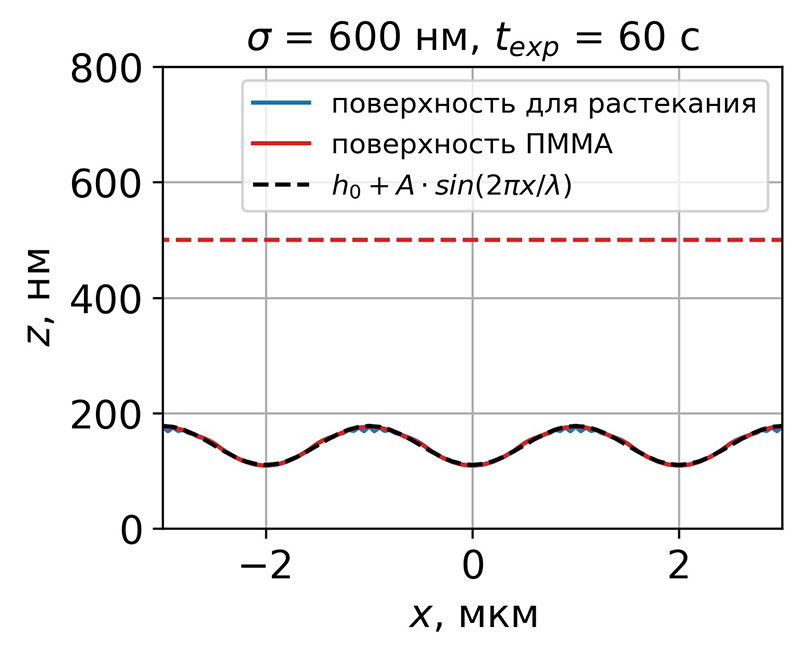
\includegraphics[width=\linewidth]{DEBER_holo/2_um/holo_1C_s600_60s_um_200} \\
			\vspace{-13em} \\ \text{\hspace{-0.1em} г}) \\ \vspace{13em}
		\end{minipage}
	\vspace{-3em}
	\caption{Промоделированные синусоидальные профили с пространственным периодом $\lambda$ = 2~мкм, полученные методом СЭЛТР в слое ПММА с начальной толщиной 500 нм. Температура образцов при экспонировании -- 150~$^\circ$C, ток экспонирования -- 4.56 нА, распределение плотности тока в пучке считается нормальным со среднеквадратичным отклонением $\sigma$. Значения $\sigma$ и $t_\mathrm{exp}$ были подобраны для получения синусоидального профиля. После экспонирования образец а) охлаждался со скоростью 10~$^\circ$C/с, образцы б)--г) -- со скоростью 1~$^\circ$C/с. Черная пунктирная линия обозначает аппроксимацию промоделированного профиля функцией синус.}
	\label{fig:DEBER_holo_2um}
\end{figure}


% 1 um
\begin{figure}[t!]
	\begin{minipage}{0.48\textwidth}
		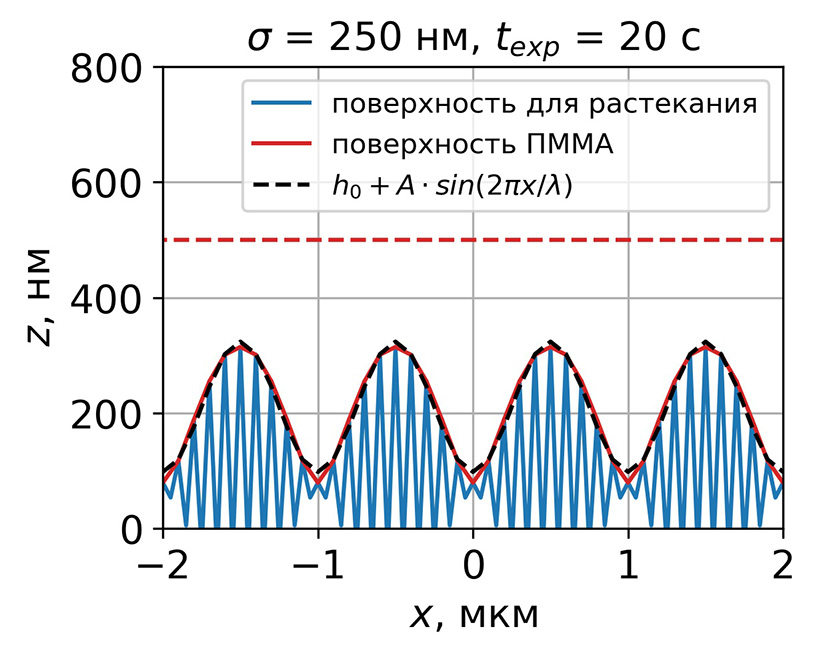
\includegraphics[width=\linewidth]{DEBER_holo/1_um/holo_1C_s250_20s_um_200} \\
		\vspace{-13em} \\ \text{\hspace{0em} a}) \\ \vspace{13em}
	\end{minipage}
	\begin{minipage}{0.48\textwidth}
		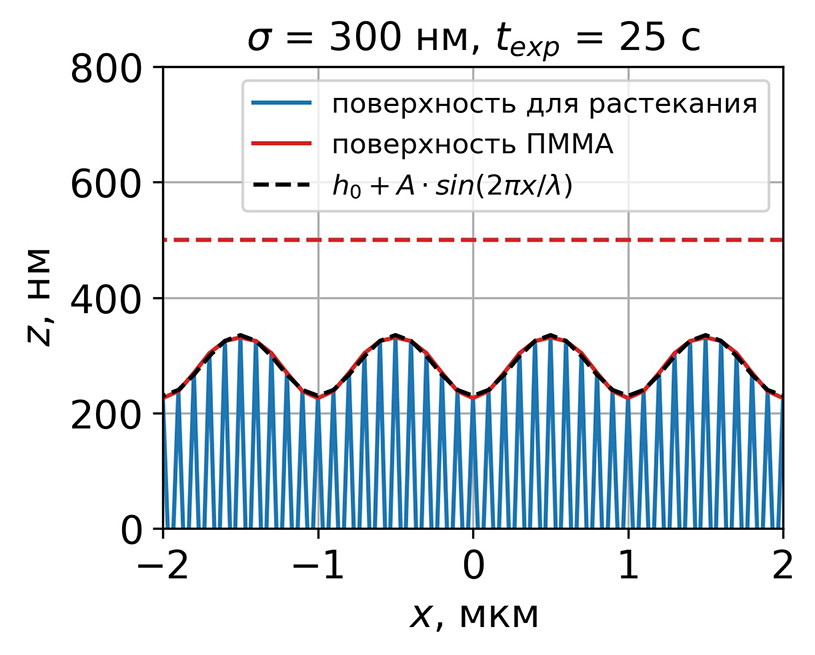
\includegraphics[width=\linewidth]{DEBER_holo/1_um/holo_5C_s300_25s_um_200} \\
		\vspace{-13em} \\ \text{\hspace{-0.1em} б}) \\ \vspace{13em}
	\end{minipage}
	\vspace{-3em}
	\caption{Промоделированные синусоидальные профили с пространственным периодом $\lambda$ = 1~мкм, полученные методом СЭЛТР в слое ПММА с начальной толщиной 500 нм. Температура образцов при экспонировании -- 150~$^\circ$C, ток экспонирования -- 4.56 нА, распределение плотности тока в пучке считается нормальным со среднеквадратичным отклонением $\sigma$. Значения $\sigma$ и $t_\mathrm{exp}$ были подобраны для получения синусоидального профиля. После экспонирования образец а) охлаждался со скоростью 1~$^\circ$C/с, образец б) -- со скоростью 5~$^\circ$C/с. Черная пунктирная линия обозначает аппроксимацию промоделированного профиля функцией синус.}
	\label{fig:DEBER_holo_1um}
\end{figure}


% 0.6 um
\begin{figure}[t!]
	\begin{minipage}{0.48\textwidth}
		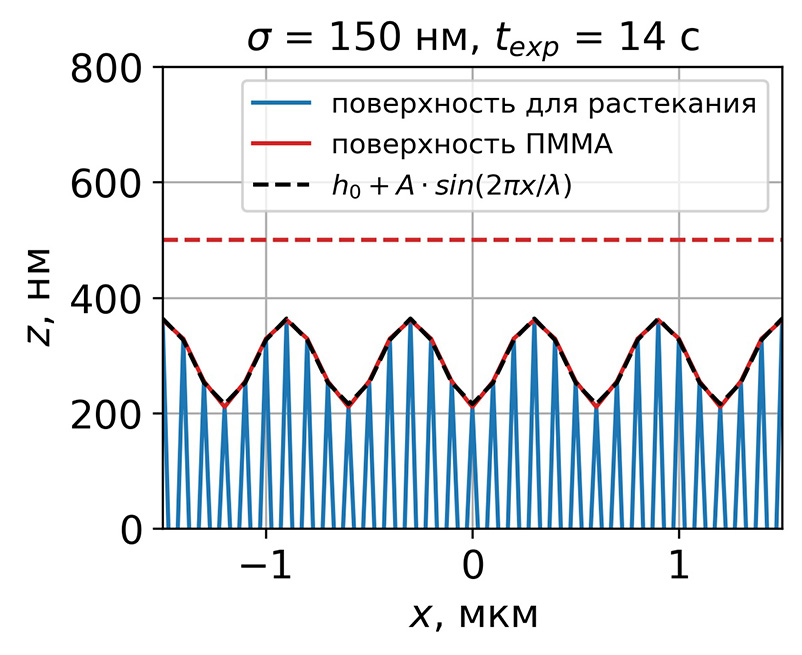
\includegraphics[width=\linewidth]{DEBER_holo/0p6_um/holo_10C_s150_14s_um_200} \\
		\vspace{-13em} \\ \text{\hspace{0em} a}) \\ \vspace{13em}
	\end{minipage}
	\begin{minipage}{0.48\textwidth}
		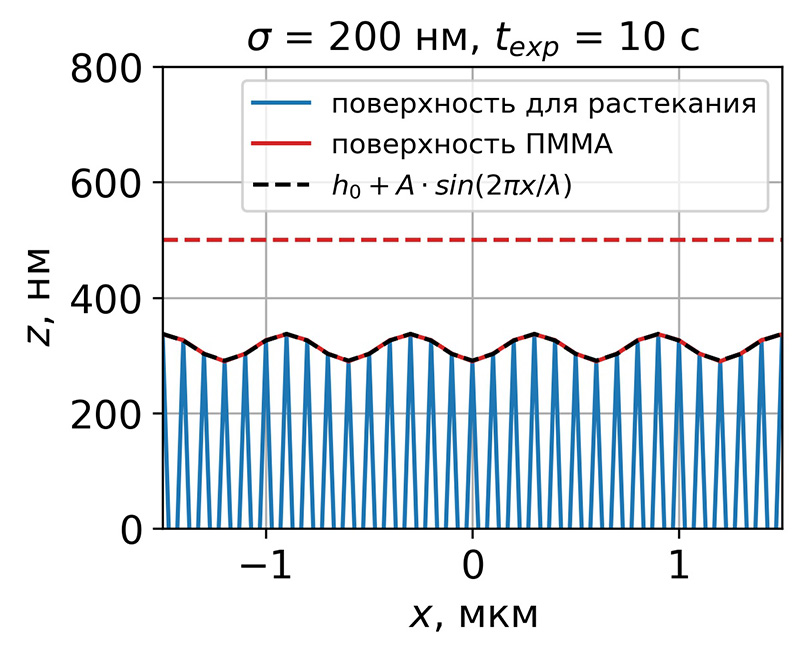
\includegraphics[width=\linewidth]{DEBER_holo/0p6_um/holo_2C_s200_10s_um_200} \\
		\vspace{-13em} \\ \text{\hspace{-0.1em} б}) \\ \vspace{13em}
	\end{minipage}
	
	\vspace{-3em}
	\caption{Промоделированные синусоидальные профили с пространственным периодом $\lambda$ = 0.6~мкм, полученные методом СЭЛТР в слое ПММА с начальной толщиной 500 нм. Температура образцов при экспонировании -- 150~$^\circ$C, ток экспонирования -- 4.56 нА, распределение плотности тока в пучке считается нормальным со среднеквадратичным отклонением $\sigma$. Значения $\sigma$ и $t_\mathrm{exp}$ были подобраны для получения синусоидального профиля. После экспонирования образец а) охлаждался со скоростью 10~$^\circ$C/с, образец б) -- со скоростью 2~$^\circ$C/с. Черная пунктирная линия обозначает аппроксимацию промоделированного профиля функцией синус.}
	\label{fig:DEBER_holo_0p6um}
	\vspace{2em}
\end{figure}
